\textbf{See the instruction for questions \inteval{\value{question}+1} to \inteval{\value{question}+2}.}

\begin{figure}[H]
\centering
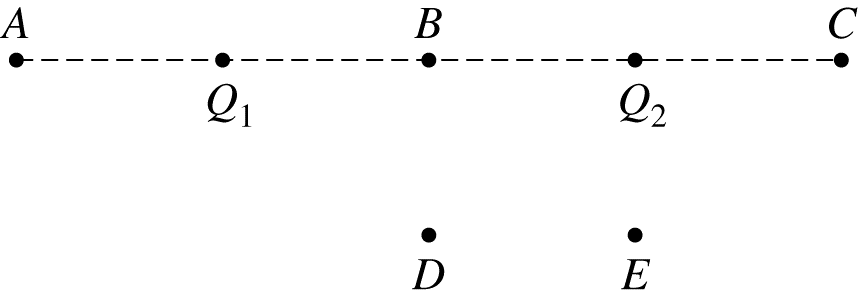
\includegraphics[scale=0.25]{images/img-011-033.png}
\end{figure}

Two point charges, $Q_{1}=+3 \unit{\mu C}$ and $Q_{2}=-3 \unit{\mu C}$, are situated as shown in the figure above.

% Multiple Choice Question 21
\begin{questions}\setcounter{question}{20}\question
At which labeled point is the magnitude of the electric field greatest?

\begin{oneparchoices}
\choice $A$
\choice $B$
\choice $C$
\choice $D$
\choice $E$
\end{oneparchoices}\end{questions}

% Multiple Choice Question 22
\begin{questions}\setcounter{question}{21}\question
At which labeled point is the electric potential the lowest?

\begin{oneparchoices}
\choice $A$
\choice $B$
\choice $C$
\choice $D$
\choice $E$
\end{oneparchoices}\end{questions}

